\documentclass[12pt]{article}
\usepackage{graphicx}
\usepackage {color}
\usepackage{pdfpages}
\usepackage{float}
\usepackage{changebar}
\usepackage{enumitem,amssymb}
\renewcommand{\familydefault}{\sfdefault}
\usepackage[margin=1.2in]{geometry}
\usepackage{graphicx}
\usepackage{wrapfig}
\usepackage[super]{cite}
\usepackage{subcaption}
\usepackage[table]{xcolor}
\usepackage{amsmath}
\usepackage[sort, numbers]{natbib}
\usepackage{multirow}
\usepackage{tabularx}
\usepackage{siunitx}

%%%%%%%%%%%%Defining the margins %%%%%%%%%%%%%%%%%%%%%
\textheight 9.in
\textwidth 6.5in
\topmargin -.5in
\oddsidemargin 0in
\setlength{\parskip}{\smallskipamount}

%%%%%%%%%%%%%%Specific Commands %%%%%%%%%%%%%%%%%%
\newcommand{\eg}{{\em e.g.,}}
\newcommand{\ie}{{\em i.e.,}}
\newcommand{\etc}{{\em etc.,}}
\newcommand{\etal}{{\em et al.}}
\newcommand{\degrees}{{$^{\circ}$}}
\newcommand{\fig}[1]{Figure~\ref{#1}}
\newcommand{\spo}{{SPO$_2$}}
%%%%%%%%%%%%%%%%%%%%%%%%%%%% Setting to control figure placement
% These determine the rules used to place floating objects like figures 
% They are only guides, but read the manual to see the effect of each.
\renewcommand{\topfraction}{.9}
\renewcommand{\bottomfraction}{.9}
\renewcommand{\textfraction}{.1}
\renewcommand{\familydefault}{\sfdefault} %setting the san serif font

%%%%%%%%%%%%%%%%%%%%%%%% Line spacing
% Use the following command for ``double'' spacing
%\setlength{\baselineskip}{1.2\baselineskip}
% and this one for an acceptable NIH spacing of 6lpi based on 11pt
%\setlength{\baselineskip}{.9\baselineskip}
% The baselineskip does not appear to work when we include a maketitle
% command in the main file.  Something there must set the line spacing
% If we use this next command, then things seem to work.
\renewcommand{\baselinestretch}{.9}

\setcounter{secnumdepth}{0} %make no numbers but have a table of contents


\begin{document}

\title{Lab 5: Exercise Stress}
\author{Jake Bergquist, u6010393, Partners: Bram Hunt,  }
\maketitle

\section{Introduction}
In this laboratory exercise we set out to investigate the methodology by which blood pressure is measured externally, observe the various externally apparent features of the venous system, and investigate the effects of exercise on the parameters of blood pressure, heart rate, and ECG presentation. The ability to monitor blood pressure externally has been used diagnostically by physicians for many years. With the use of a blood pressure cuff and a stethoscope a physician can quickly assess the diastolic and systolic blood pressure using deflections of the pressure cuff and the sound of turbulent blood flow. Properties of the venous structure can also be characterized from external observation, such as the direction of flow and functioning of the valves. Our main goal was to utilize the blood pressure, and heart rate measures, along with a recorded ECG, to characterize the repose of the body to exercise. We chose to implement a model in which the subject either exercised intensely or moderately in short bursts followed by rest periods to characterize the response tot he exercise as well as the subsequent recovery. This investigation will show changes in ECG, blood pressure, and heart rate. We expect that blood pressure and heart rate should increase during exercise however the response may vary during sequential exercise periods. If the exercise is intense we expect that the parameters of blood pressure and heart rate will not be able to recover as well as when the exercise periods are moderate.


\section{Methods}

\subsection{Blood Pressure Measurement}
To assess blood pressure a blood pressure cuff was attached tot he left arm of the subject and inflated. The systolic pressure is first measured by inflating the cuff to block flow then slowly letting off low until the radial pulse returns by palpation. This also corresponds t a bump in pressure seen on the pressure gauge. The pressures were then taken again by inflating the cuff to cut of flow and a stethoscope was placed over the antecubital fossa. The pressure was released until a sound of blood flow returned (which was confirmed as the systolic pressure by the bump on the pressure gauge), and again until the sound stopped (diastolic pressure).

\subsection{Examination of Venous Function}
The subject was laid on the ground and a suitable set of veins was identified on the feet which were distinctly visible. The feet of the subject were raised above the heart until the point where they just barely collapsed. This distance was measured and used to calculate the venous pressure. A vein was then indentified on the hand of the subject and the flow was blocked manually.  The blood int he vein was then pressed towards and away from the block and released and the response was observed.

\subsection{Exercise Stress}
The subject was fit with four recording electrodes, one ont he left pectoral muslce (LA), one of the right pectoral muslce (RA), one on the left bottom of the rib cage between two ribs (LL) , one on the right bottom of the rib cage between two ribs (RL). RA, LA, and LL formed the standard limb lead configuration and RL served as a reference. Recording and exercise were performed according to Figure~\ref{fig:Protocol}. Before each phase a 30 second baseline ECG was taken along with a baseline hear rate, SP02, and blood pressure. In phase one the subject was instructed to peddle on the bike a maximu intensity (roughly 130 beats per minute on a metronome to time the pace of each peddle). Exercise was performed in 45 second intervals followed by 90 second rest periods. During the rest period blood pressure is measured as soon as possible, continuous ECG is recorded, and SP02 and heart rate are recorded every 10 to 15 seconds. Phase two is performed 30 minutes after phase one once the subject has fully recovered. Phase two follows the protocol of phase one witht he exception that the exercise intensity is reduced to be moderate with a pace of roughly 80 bpm for each pedal.

\begin{figure}[H]
	
	\centering
	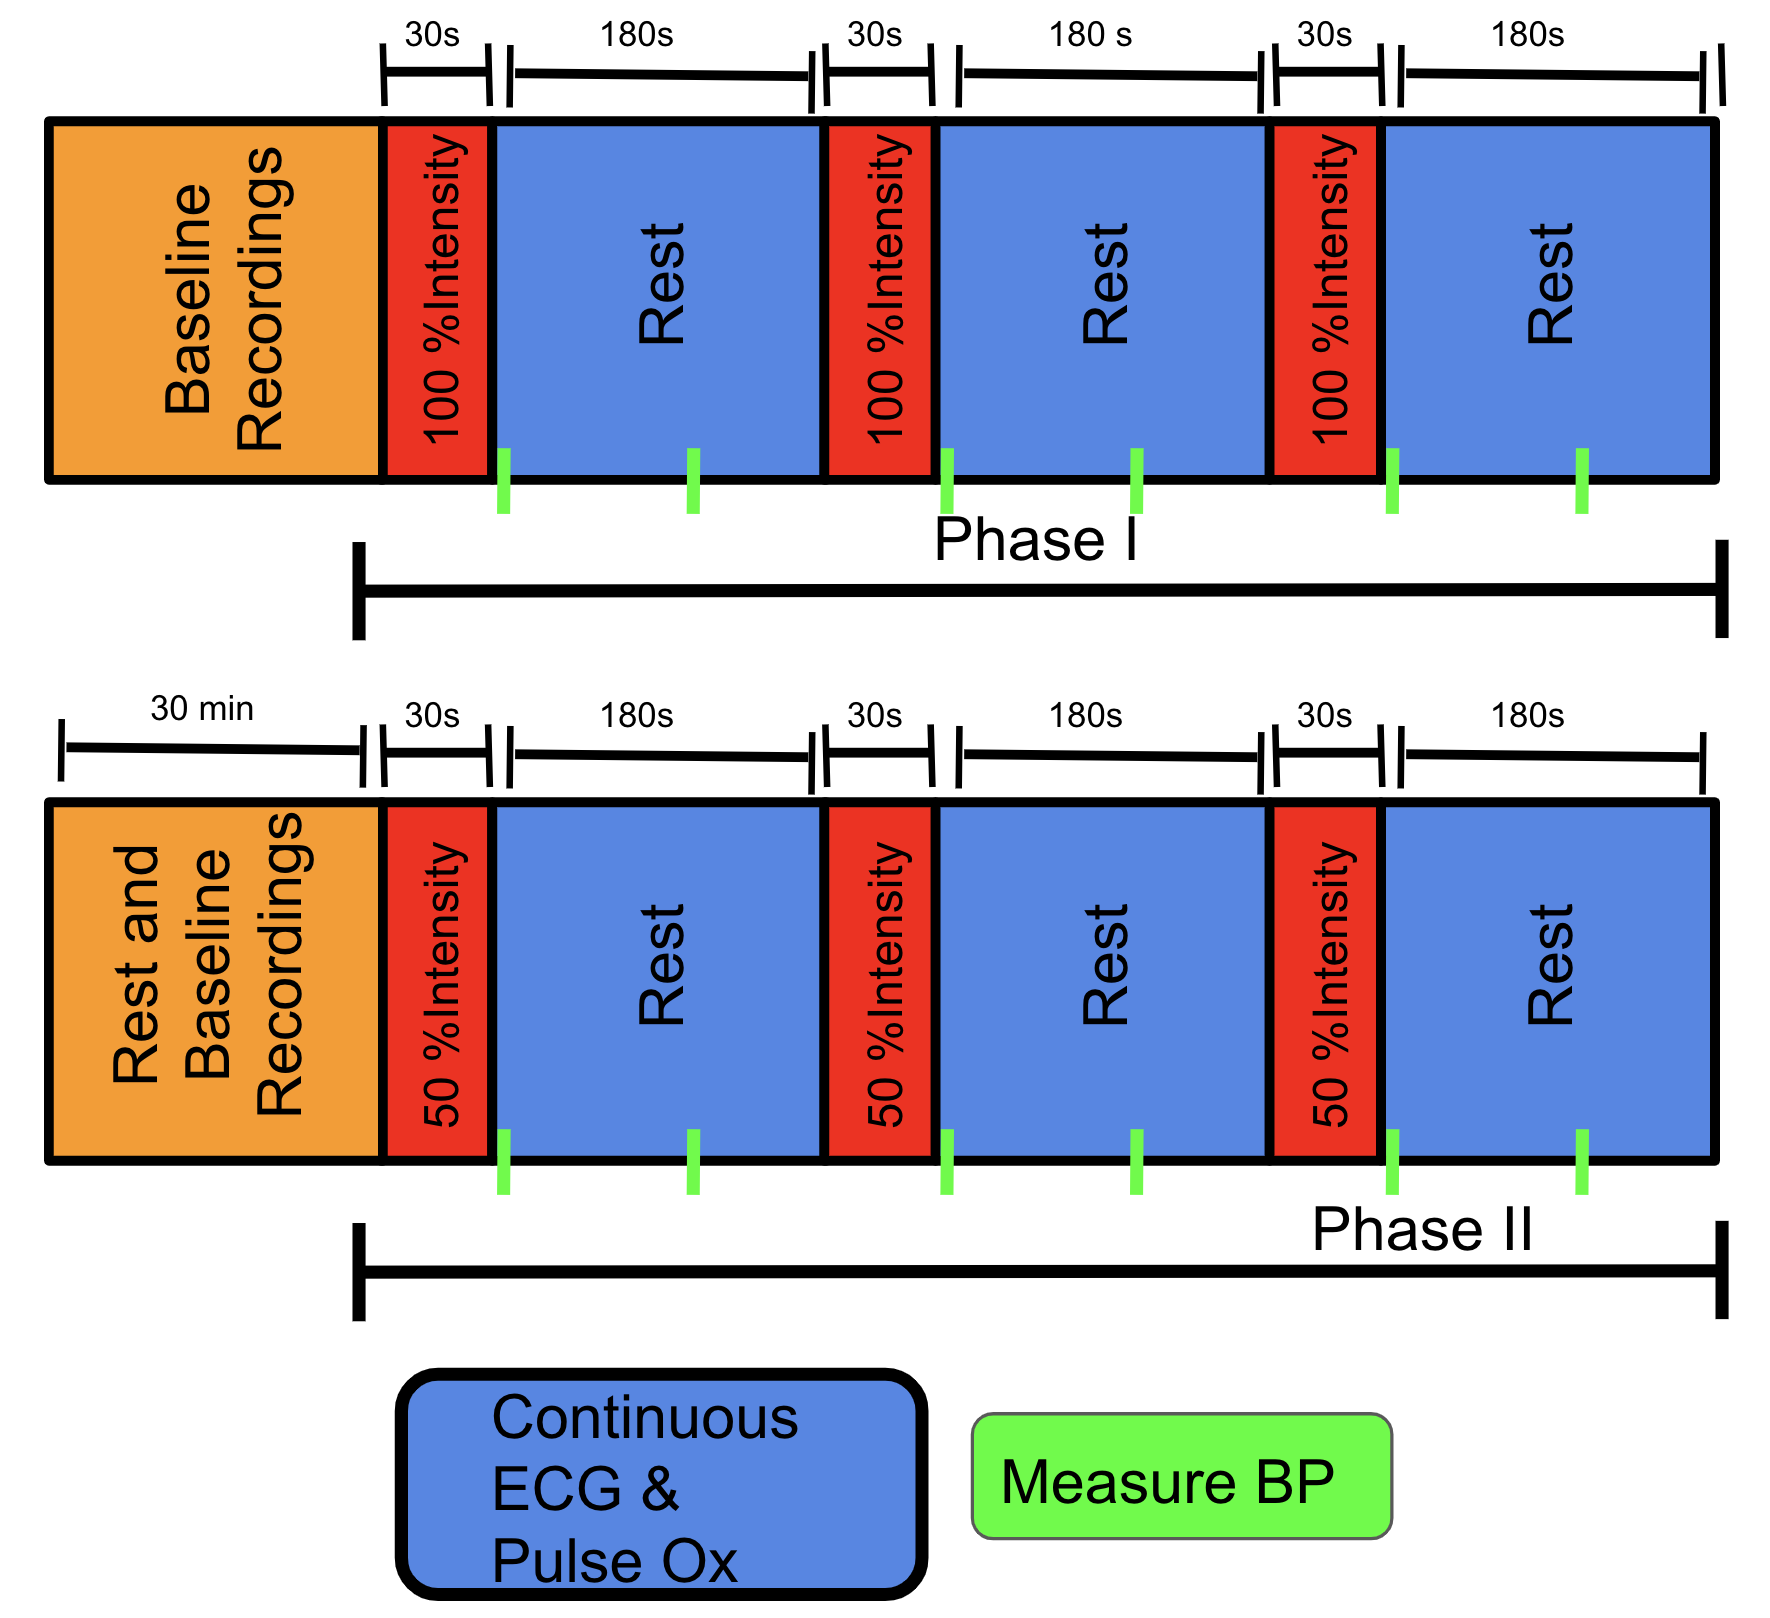
\includegraphics[width = .8\textwidth]{Figures/protocol.png}
	\caption{}
	\label{fig:Protocol}
\end{figure}

\subsection{Processing}
The recorded ECG data was processed using PFEIFER, a preprocessing framework for electrograms, that filters, baseline corrects, fiducilizes, auto fiducilizes, and time aligns the signals.\cite{MacLeod2018_p} Signals were assessed for qualitative differences during each recovery period and interesting changes were hilighted in the results.

\section{Results}
Using the palpatory method we measured a systolic blood pressure of 110 mmHg. Utilizing the Auscultatory method we could not quite distinguish when the non laminar sounds (Korotkow's sounds) started and stopped, however we were able to take the combined method measurements. This produced a systolic (when radial pulse returns) pressure of 110 mmHg, and a diastolic (first sound of Korotkow's sounds) pressure of 85 mmHg.

Before either exercise protocol the resting heart rate was 84 bpm and the \spo{} was 
\section{Discussion}

%%%%%%%%%%%%%%%%%% Correct Bibliography Style

\bibliography{C:/Users/Jake/Documents/library}
\bibliographystyle{IEEEtran}


\end{document}








